\documentclass[tikz,border=10pt]{standalone}
\usepackage{amsmath,amssymb}
\usepackage{pgfplots}
\pgfplotsset{compat=1.18}
\usetikzlibrary{arrows.meta,positioning,calc,shapes,fit,backgrounds}

\definecolor{politoNavy}{RGB}{0, 43, 91}
\definecolor{deepdiveTeal}{RGB}{0, 128, 128}
\definecolor{examred}{RGB}{180, 40, 40}
\definecolor{intuitiongreen}{RGB}{40, 130, 80}
\definecolor{cardBack}{RGB}{250, 250, 252}

\begin{document}
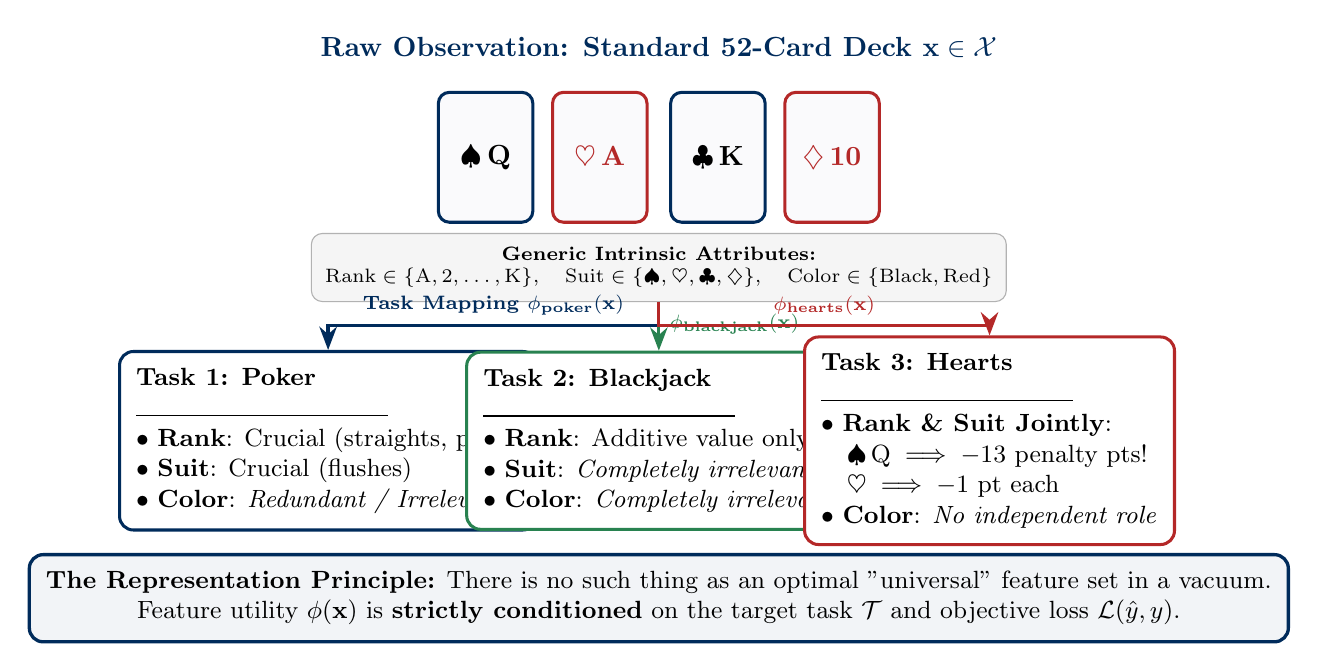
\begin{tikzpicture}[>=Stealth, node distance=1.2cm, scale=1.0]
  % Styles
  \tikzstyle{card} = [draw=politoNavy, fill=cardBack, rounded corners=4pt, minimum width=1.2cm, minimum height=1.65cm, line width=1.1pt, font=\bfseries]
  \tikzstyle{taskbox} = [draw=deepdiveTeal, fill=white, rounded corners=5pt, line width=1.1pt, inner sep=6pt, font=\small, align=left]

  % Raw Playing Cards Deck
  \node[font=\bfseries\normalsize, text=politoNavy] (title) at (0, 3.2) {Raw Observation: Standard 52-Card Deck $\mathbf{x} \in \mathcal{X}$};

  % Visual Cards
  \node[card] (c1) at (-2.2, 1.8) {$\spadesuit$\,\text{Q}};
  \node[card, draw=examred, text=examred] (c2) at (-0.75, 1.8) {$\heartsuit$\,\text{A}};
  \node[card] (c3) at (0.75, 1.8) {$\clubsuit$\,\text{K}};
  \node[card, draw=examred, text=examred] (c4) at (2.2, 1.8) {$\diamondsuit$\,10};

  % Intrinsic Features Panel
  \node[draw=gray!60, fill=gray!8, rounded corners=4pt, inner sep=5pt, font=\scriptsize, align=center] (feat) at (0, 0.4) {
    \textbf{Generic Intrinsic Attributes:}\\
    $\text{Rank} \in \{\text{A}, 2, \dots, \text{K}\}, \quad \text{Suit} \in \{\spadesuit, \heartsuit, \clubsuit, \diamondsuit\}, \quad \text{Color} \in \{\text{Black}, \text{Red}\}$
  };

  % Downstream Task Nodes
  \node[taskbox, draw=politoNavy] (t1) at (-4.2, -1.8) {
    \textbf{Task 1: Poker}\\
    \rule{3.2cm}{0.4pt}\\
    $\bullet$ \textbf{Rank}: Crucial (straights, pairs)\\
    $\bullet$ \textbf{Suit}: Crucial (flushes)\\
    $\bullet$ \textbf{Color}: \textit{Redundant / Irrelevant}
  };

  \node[taskbox, draw=intuitiongreen] (t2) at (0, -1.8) {
    \textbf{Task 2: Blackjack}\\
    \rule{3.2cm}{0.4pt}\\
    $\bullet$ \textbf{Rank}: Additive value only\\
    $\bullet$ \textbf{Suit}: \textit{Completely irrelevant}\\
    $\bullet$ \textbf{Color}: \textit{Completely irrelevant}
  };

  \node[taskbox, draw=examred] (t3) at (4.2, -1.8) {
    \textbf{Task 3: Hearts}\\
    \rule{3.2cm}{0.4pt}\\
    $\bullet$ \textbf{Rank \& Suit Jointly}:\\
    \quad $\spadesuit\,\text{Q} \implies -13$ penalty pts!\\
    \quad $\heartsuit \implies -1$ pt each\\
    $\bullet$ \textbf{Color}: \textit{No independent role}
  };

  % Connecting Arrows
  \draw[->, very thick, politoNavy] (feat.south) -- ++(0, -0.3) -| (t1.north) 
    node[pos=0.25, above, font=\scriptsize\bfseries, text=politoNavy] {Task Mapping $\phi_{\text{poker}}(\mathbf{x})$};
  \draw[->, very thick, intuitiongreen] (feat.south) -- (t2.north)
    node[pos=0.45, right, font=\scriptsize\bfseries, text=intuitiongreen] {$\phi_{\text{blackjack}}(\mathbf{x})$};
  \draw[->, very thick, examred] (feat.south) -- ++(0, -0.3) -| (t3.north)
    node[pos=0.25, above, font=\scriptsize\bfseries, text=examred] {$\phi_{\text{hearts}}(\mathbf{x})$};

  % Core Moral Callout
  \node[draw=politoNavy, fill=politoNavy!5, rounded corners=5pt, line width=1.2pt, font=\small, align=center, inner sep=6pt] at (0, -3.8) {
    \textbf{The Representation Principle:} There is no such thing as an optimal "universal" feature set in a vacuum.\\
    Feature utility $\phi(\mathbf{x})$ is \textbf{strictly conditioned} on the target task $\mathcal{T}$ and objective loss $\mathcal{L}(\hat{y}, y)$.
  };
\end{tikzpicture}
\end{document}
